\documentclass{standalone}
\usepackage{tikz}
\usetikzlibrary{positioning}

\begin{document}

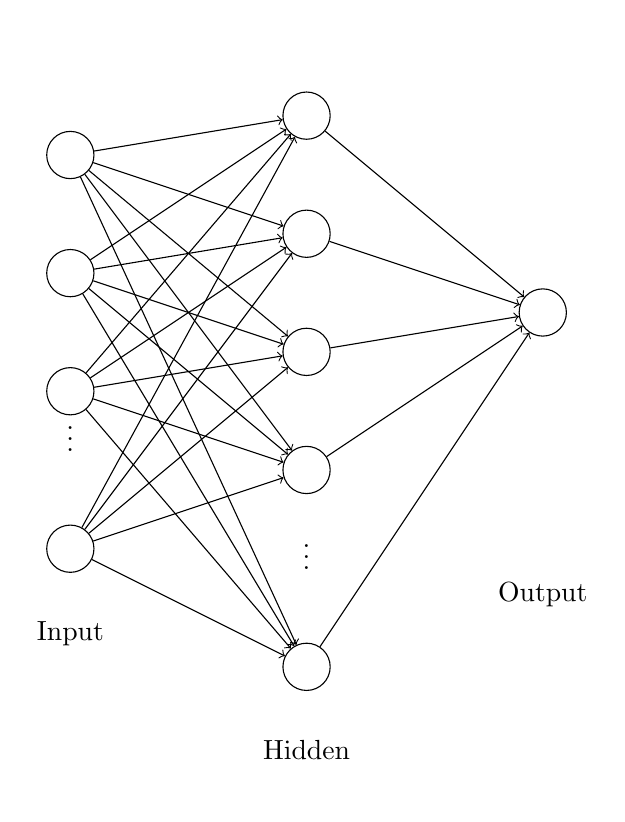
\begin{tikzpicture}[scale=1, every node/.style={transform shape}]
    % Input layer
    \foreach \i in {1,2,3}
        \node[circle, draw, minimum size=6mm, inner sep=0pt] (I-\i) at (0, -\i*1.5 -1) {};
    \node[draw=none] (I-4) at (0, -6) {\vdots};
    \node[circle, draw, minimum size=6mm, inner sep=0pt] (I-5) at (0, -7.5) {};
    \node[below=0.5cm of I-5, draw=none] (ILabel) {Input};

    % Hidden layer
    \foreach \i in {1,2,3,4}
        \node[circle, draw, minimum size=6mm, inner sep=0pt] (H-\i) at (3, -\i*1.5 -0.5) {};
    \node[draw=none] (H-5) at (3, -7.5) {\vdots};
    \node[circle, draw, minimum size=6mm, inner sep=0pt] (H-6) at (3, -9) {};
    \node[below=0.5cm of H-6, draw=none] (HLabel) {Hidden};

    % Output layer
    \node[circle, draw, minimum size=6mm, inner sep=0pt] (O-1) at (6, -4.5) {};
    \node[below=3cm of O-1, draw=none] (OLabel) {Output};

    % Connect layers
    \foreach \i in {1,2,3,5}
        \foreach \j in {1,2,3,4,6}
            \draw[->] (I-\i) -- (H-\j);

    \foreach \i in {1,2,3,4,6}
        \draw[->] (H-\i) -- (O-1);

    % Add margins using transparent nodes
    \node[draw=none] (margin-top) at (0, -1) {};
    \node[draw=none] (margin-bottom) at (0, -10.5) {};
\end{tikzpicture}

\end{document}
